
%(BEGIN_QUESTION)
% Copyright 2006, Tony R. Kuphaldt, released under the Creative Commons Attribution License (v 1.0)
% This means you may do almost anything with this work of mine, so long as you give me proper credit

Svar på følgende spørsmål om denne analoge proporsjonalregulatorkretsen:

$$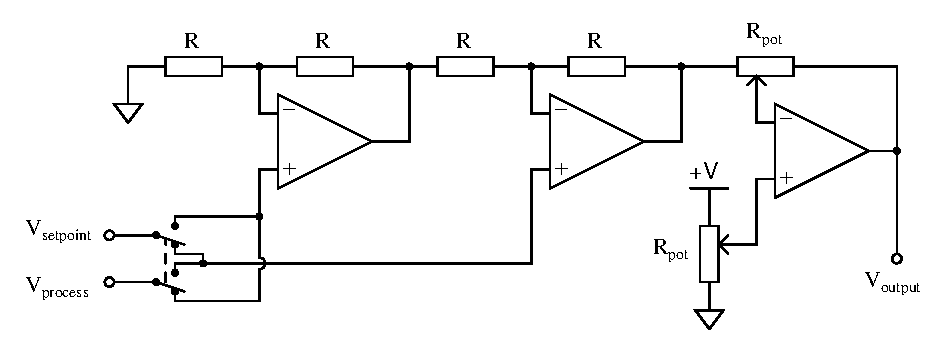
\includegraphics[width=15.5cm]{i01494x01.eps}$$

\begin{itemize}
\item{} Hvordan justeres proporsjonalbåndinnstillingen?
\vskip 10pt
\item{} Hvordan justeres bias-innstillingen?
\vskip 10pt
\item{} Hvilken bryterstilling gir {\it direkte} virkning, og hvilken gir {\it omvendt} virkning?
\vskip 10pt
\item{} Beregn proporsjonalbåndet for denne kretsen dersom alle $R$-verdier er helt like, og begge potensiometrene står i midtstilling.
\end{itemize}

\vfil

\underbar{file i01494}
\eject
%(END_QUESTION)





%(BEGIN_ANSWER)

Dette er en vurderingsoppgave -- ingen svar eller hint oppgis!

%(END_ANSWER)





%(BEGIN_NOTES)

Vi vet at {\it proporsjonalbånd} er relatert til regulatorens {\it gain}, og derfor vil potensiometeret som setter gain (forsterkning) i denne kretsen være proporsjonalbåndjusteringen. Dette kan bare være potensiometeret i tilbakekoblingsnettet til den siste op-ampen.

\vskip 10pt

Vi vet at {\it bias} er en additiv størrelse til utgangen ($m$) i en sløyferegulator. Derfor må vi se etter et potensiometer i kretsen som forskyver utgangsspenningen. I dette tilfellet er det potensiometeret koblet som spenningsdeler til den ikke-inverterende inngangen på den siste op-ampen.

\vskip 10pt

{\it Direkte virkning} er definert som at utgangen fra en sløyferegulator øker når prosessvariabelen (PV) øker, mens {\it omvendt virkning} er definert som at utgangen synker når prosessvariabelen (PV) øker. Vi kan avgjøre hvilken bryterstilling som gir hvilken virkning ved å bruke ``tankeeksperimenter'', der vi forestiller oss at $V_{process}$ øker, og så bestemmer hvilken retning $V_{output}$ går. Med bryteren slik den er vist i figuren, registreres økende $V_{process}$ på den ikke-inverterende inngangen til første op-amp, og denne utgangen går opp. Dette stigende signalet går inn på inverterende inngang i neste op-amp, som derfor får utgangen sin ned. Dette signalet går igjen inn på inverterende inngang i siste op-amp, og dermed går $V_{output}$ opp. Derfor er bryterstillingen som vist i figuren {\it direktevirkende}.

\vskip 10pt

Hvis alle $R$-verdier er like og begge potensiometre står i midten, får regulatoren total gain på 2 (P.B. = 50\%). Den siste op-ampen (til høyre) er en inverterende forsterker med gain 1 når inngangs- og tilbakekoblingsmotstand er like i tilbakekoblingsnettet. De to andre op-ampene er konfigurert som ikke-inverterende forsterkere (med hensyn til PV- og SP-inngangene) med gain 2 når motstandene i tilbakekoblingsnettene har like verdier.

%INDEX% Control, proportional: analog electronic controller

%(END_NOTES)

